\subsection{Cross Sections as a function of Acoplanarity}

The differential cross section as a function of $\phi_{T}$ for interactions on the CH, C, H$_{2}$O, Fe, and Pb targets, respectively, are shown in Fig.~\ref{figure:xsec_coplan}. %The data are represented by the black points with error bars.  
The simulations (MINERvA tune) are represented by the histograms and further distinguished by their respective interaction processes.
A similar format is used in the cross-section plots for each of the other variables in this section.  The uncertainties broken down by source for both the absolute cross sections and the cross section ratios as a function of $\phi_T$ can be found in Fig.~\ref{fig:xsec_err_coplan}.

% tki_coplanar xsecs
\begin{figure}[h]  
	\centering
 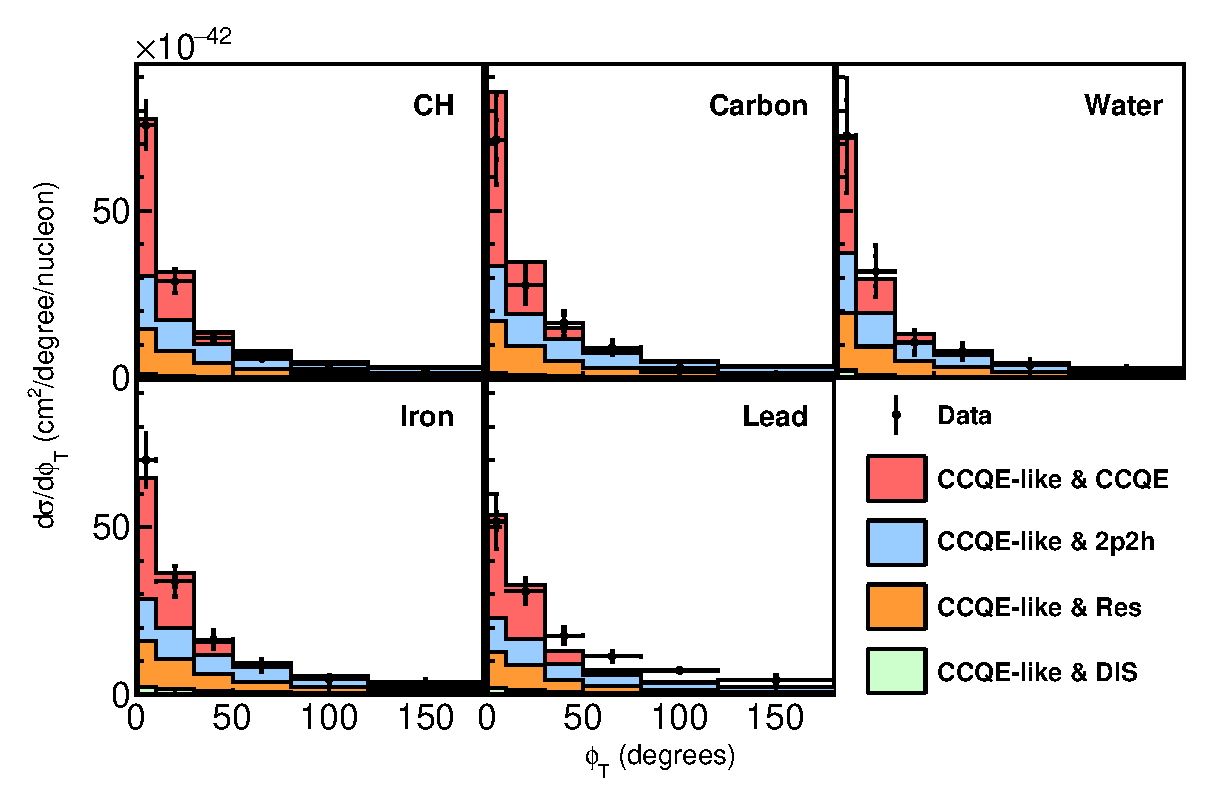
\includegraphics[width=\linewidth]{Figures/xsec_five_square/phi.eps}
	\caption{The differential cross section as a function of $\phi_{T}$ for CH, C, H$_{2}$O, Fe, and Pb targets, along with the predictions for the different quasielastic-like signal processes.}
	\label{figure:xsec_coplan}
\end{figure}

%$\phi_{T}$ is the supplementary angle to the coplanarity, i.e., 180$^{\circ}$-coplanarity. 

The variable $\phi_{T}$ (see Fig.~\ref{fig:TKI}) is a measure of the extent to which the proton momentum is not back-to-back with the muon momentum in the transverse plane.  Such a deviation from back-to-back might be expected to happen with the effects of FSI as the proton transits the nucleus.  From the way that $\phi_{T}$ is defined, a larger value means more of a deviation from back-to-back and the greater the FSI effects.  The MINERvA tune shown uses a GENIE2 hA FSI model which does not change the angular distribution of the outgoing protons from quasielastic interactions for larger nuclei, but a full cascade like hN would broaden the angular distributions.   The prevalence of resonance feed-in to the signal in this model is also not strongly modified with A.   
The most noticeable difference between the data and the simulation is in the case of the Pb target where there is significantly more cross section at larger $\phi_{T}$, indicating more FSI broadening in the data.

The differential cross section as a function of $\phi_{T}$ for the different targets as compared to a range of models is given in Fig.~\ref{fig:models_coplan}. As seen earlier, NEUT appears to have a higher cross section than seen in the data.  The hN versions of GENIE are very similar to NEUT in the larger targets and predict more events at higher $\phi_{T}$ where the FSI effect is largest.  The \chisq\ between the cross sections and the models can be found in Table~\ref{tab:phi}.

%Here it can be seen that MnvGENIE gives the smallest cross section at low coplanarity for Pb interactions and that the other models give better agreement with the data, albeit with a large spread.  

% comparisons to generators TKI coplanarity
\begin{figure}[h]
    \centering
 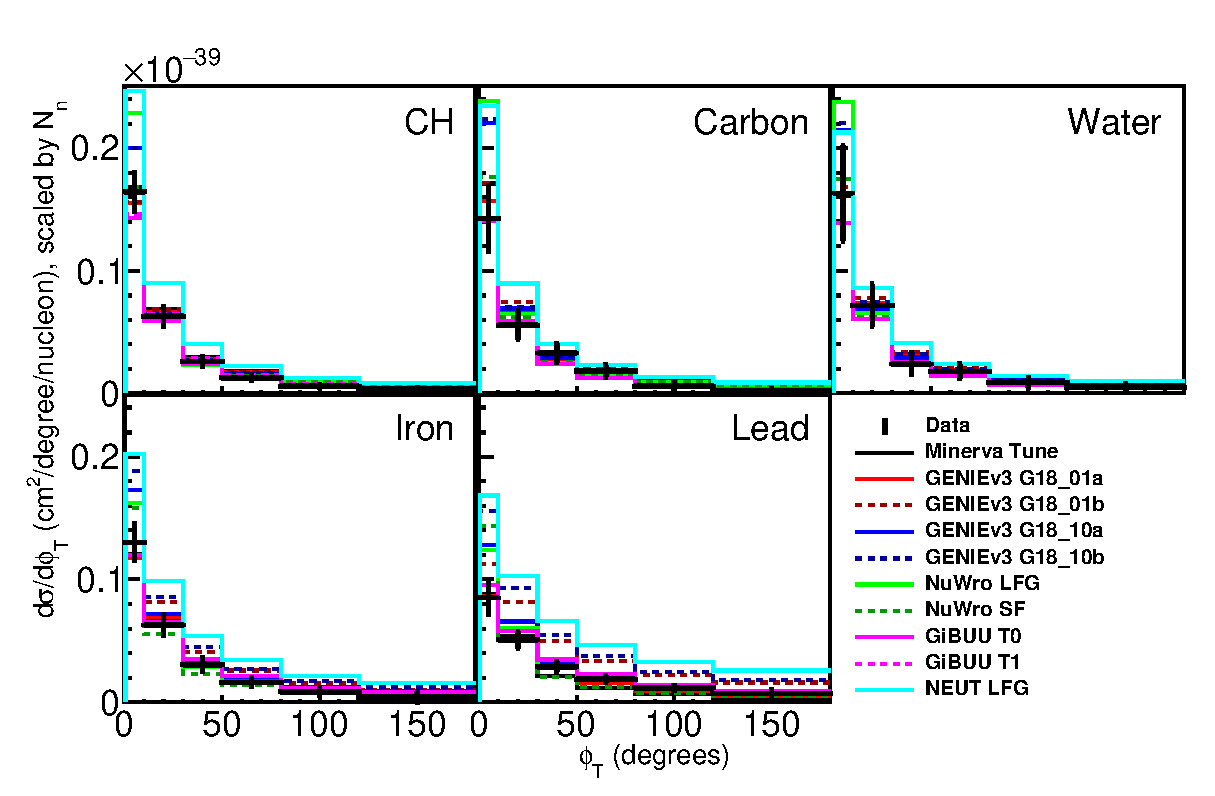
\includegraphics[width=\linewidth]
 {Figures/gencompare/phi_5square.eps}
    \caption[$\phi_{T}$ cross-section comparison for multiple targets ]{Cross section measurements and predictions as a function of $\phi_T$ for different targets and for a selection of different generator and model choices.
    }
    \label{fig:models_coplan}
\end{figure}

The ratio of the differential cross section as a function of the $\phi_{T}$ for each nuclear target (C, H$_{2}$O, Fe, Pb) to that for scintillator is shown in Fig.~\ref{Figure:Gencompare_phi_ratio}. The 
models describe the data fairly well for the smaller targets.  The model variation is greatest for the larger targets at high $\phi_{T}$.  The MINERvA tune, NuWro, and the hA versions of GENIE underpredict the ratio in the data taken on Pb at higher $\phi_{T}$.  The \chisq\ between the cross section ratios and the models can be found in Table~\ref{tab:phi}.  The ratio between the measured cross section and the MINERvA tune, along with the ratio between the various models and the MINERvA tune can be found in Fig.~\ref{fig:models_coplan_rat}.


 

\begin{figure}
    \centering
            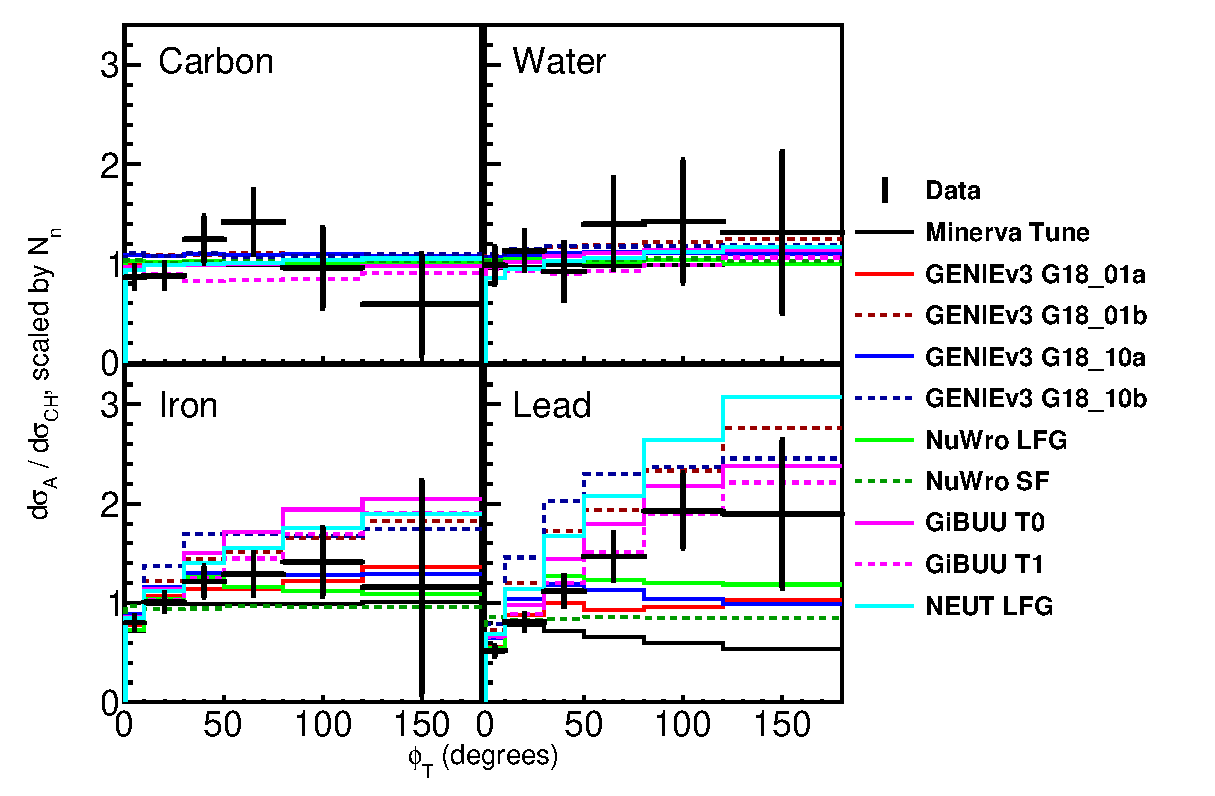
\includegraphics[width=\linewidth] {Figures/gencompare/phi_4square.eps}
    \caption{$\phi_{T}$ cross-section ratio comparison for multiple targets. Note that changes to the FSI model (GENIE ``a'' to ``b'')
     in GENIE change the cross section ratio at high $\phi_T$  much more than changes to the 2p2h model (GiBUU T0 to GiBUU T1) or changes to the initial state (GENIE 1 to GENIE 10) or (NuWro LFG to NuWro SF). }
        \label{Figure:Gencompare_phi_ratio}
\end{figure}